\documentclass[tikz]{standalone}
\usepackage{tikz}
\usetikzlibrary{decorations.pathreplacing}
\begin{document}
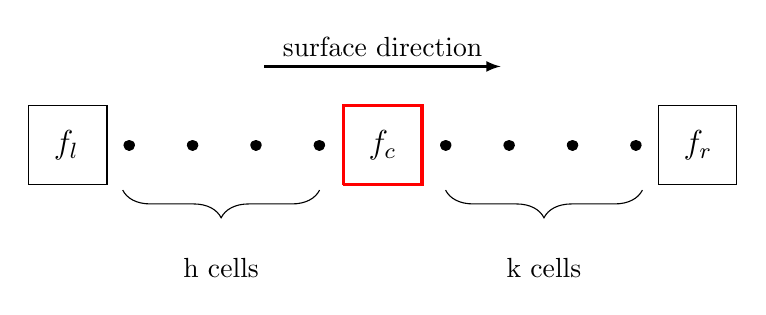
\begin{tikzpicture}[scale=1,circle dotted/.style={dash pattern=on .05mm off 8mm,line cap=round}]
  \draw (-4,0)--(-4,1)--(-3,1)--(-3,0)--(-4,0);
  \draw[very thick,red] (0,0)--(0,1)--(1,1)--(1,0)--(0,0);
  \draw (4,0)--(4,1)--(5,1)--(5,0)--(4,0);
  \draw[line width=4,circle dotted] (1.3,0.5)--(3.8,0.5);
  \draw[line width=4,circle dotted] (-0.3,0.5)--(-2.8,0.5);
  \draw[decorate,decoration={brace,amplitude=10,mirror,raise=2}] (1.3,0)--(3.8,0) node[midway,yshift=-3em] {k cells};
  \draw[decorate,decoration={brace,amplitude=10,raise=2}] (-0.3,0)--(-2.8,0) node[midway,yshift=-3em] {h cells};
  \node[anchor=west] at (0.2,0.5) {\large $f_c$};
  \node[anchor=west] at (4.2,0.5) {\large $f_r$};
  \node[anchor=west] at (-3.8,0.5) {\large $f_l$};
  \draw[thick,-latex] (-1,1.5)--(2,1.5) node[above,midway] {surface direction};
\end{tikzpicture}
\end{document}
